\section{Lab 1 - Introduction to FPGA's and VHDL}

\subsection{Introduction}
This lab will introduce you to the Altera DE2-115 FPGA Development Board. The DE2-115 contains all of the hardware necessary to prototype and create various hardware configurations on the Altera Cyclone IV FPGA chip that will be used throughout the course of this lab. By completeing this lab, you will have an understanding of all the hardware contained on the FPGA development board, along with an understanding of how to connect peripherals to the development board. Lastly, this lab will go over the standard template for designing hardware in the VHDL programming language. All this will be accomplished by following the Quartus II introductory packet along with the following activities.

\subsection{VHDL Basics}

The following code block shows how to interact with the switches and LEDs on the DE2-115. Notice how the program begins with importing the ieee library which contains all of the basic logic primitives as established within the IEEE standard 1164. When working in industry it is common for large companies to create their own libraries as well. Every VHDL file should contain at least one entity (module) that is the same as the name of the file. An entity contains information about the structure of the module such as how many inputs/outputs (I/O) and what type of logic to expect at the I/O. Finally we define the entity in an architecture block, this section does the work on the hardware. As can be seen, this code is setting the red LEDs as defined in the array to the accompanying switches on the board. Take note on the use of comments throughout the code, comments begin with two dashes (--) and should always be used to describe what you are trying to accomplish, this way someone else who reads your code will understand it easily and your code will look more professional. 

\begin{lstlisting}
-- Import logic primitives
LIBRARY ieee;
USE ieee.std_logic_1164.all;

-- Simple module that connects the SW switches to the LEDR lights
ENTITY lab1 IS
PORT ( SW: IN STD_LOGIC_VECTOR(17 DOWNTO 0); -- Initialize switches as an input
	LEDR: OUT STD_LOGIC_VECTOR(17 DOWNTO 0)); -- Initialize red LEDs as an output
END lab1;

-- Define characteristics of the entity lab1
ARCHITECTURE Behavior OF lab1 IS
BEGIN
	LEDR <= SW; -- Assign each switch to one red LED
END Behavior;
\end{lstlisting}


\subsection{Activities}

\subsubsection{Implementing Logic}

Implement the hardware from the circuit in Figure \ref{circuit1}. The inputs should come from SW[1] and SW[2] and the output should be shown on any of the available LEDs. Use the implemented circuit to test and create a truth table with your results and place it within a comment in the program file.

\begin{figure}[H]
	\centering
	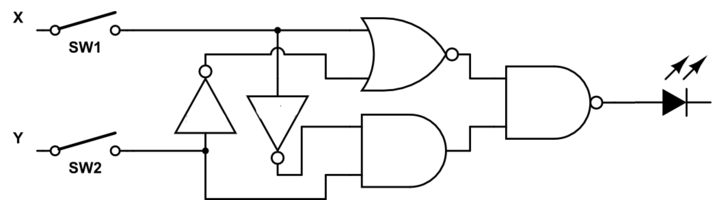
\includegraphics[width=100mm]{Lab1/figures/circuit1.png}
	\caption{Circuit for activity 1}
	\label{circuit1}
\end{figure}

\subsubsection{7-Segment Displays}
